\documentclass[10pt]{beamer}
\usepackage{amsmath}
\usepackage{amssymb}
\usepackage{bookmark}
\usepackage{hyperref}
\newcommand{\h}{\nabla^{2}}
\newcommand{\g}{\nabla}
\newcommand{\xbold}{\mathbf{x}}
\newcommand{\sbold}{\mathbf{s}}
\newcommand{\mineig}{\lambda_{\min}}
\newcommand{\maxeig}{\lambda_{\max}}
\newcommand{\eg}{\epsilon_{g}}
\newcommand{\eh}{\epsilon_{h}}
%\documentclass{article}
%\usepackage{beamerarticle}
\usetheme{CambridgeUS}

\title[Xu, Roosta-Khorasani and Mahoney]{Newton-Type Methods for Non-Convex Optimization Under Inexact Hessian Information}
\subtitle{Presented as a part of\\
CS6230 - Optimization Methods in Machine Learning}

\author{Vishwak Srinivasan \and Ayushi Patel}

\begin{document}

\begin{frame}
  \titlepage
\end{frame}

\begin{frame}{Outline}
  \tableofcontents
  % You might wish to add the option [pausesections]
\end{frame}

% Section and subsections will appear in the presentation overview
% and table of contents.
\section{Introduction}
\subsection{The problem statement}

\begin{frame}{The problem statement}
  \begin{itemize}
  \item {
    Consider a unconstrained optimization problem
    \begin{equation}
        \label{main-obj}
        \min_{\xbold \in \mathbb{R}^{d}} F(\xbold)
    \end{equation}
    where \(F : \mathbb{R}^{d} \rightarrow \mathbb{R}\), is \textit{smooth} and \textit{non-convex}.
  }
  \item<2-> {
    Many known methods to help solve the \emph{convex} version.
    \begin{itemize}
        \item First order methods
        \item Second order methods
    \end{itemize}
  }
  \item<3-> {
    First order methods are ``fine" - advances in tensor computing, automatic differentiation and so on.
    \begin{equation}
        \xbold := \xbold - \eta \g F(\xbold)
    \end{equation}
    \pause
  }
  \item<4-> {
    Are second order methods just as fine?
    \begin{equation}
        \xbold := \xbold - \eta (\h F(\xbold))^{-1} \g F(\xbold)
    \end{equation}
    \uncover<5->{How do we compute \(\h F(\xbold)\)?}
  }
  \end{itemize}
\end{frame}

\subsection{Motivation for the work}
\begin{frame}{Issues with the first order methods}
  \begin{itemize}
  \item<1->{
    Performance of first order methods can be seriously hindered by ill-conditioning.
    \begin{itemize}    
        \item<2->{Condition number: \(\kappa = \frac{L}{\gamma} = \frac{\maxeig(\h F)}{\mineig(\h F)}\), where \(L\) is smoothness parameter, \(\gamma\) is strong convexity parameter}
        \item<3->{Convergence criteria for gradient descent relies on \(\kappa\) \cite{benrecht-simons}}
    \end{itemize}
  }
  \item<4->{
    First order methods involve fine-tuning hyperparameters.
    \begin{itemize}    
        \item<5->{For gradient descent, we have 1 (learning rate) and for Adam \cite{adam-iclr} we have 4 (learning rate, tolerance, \(\beta_{1}\) and \(\beta_{2}\))}
    \end{itemize}
  }
  \item<6->{
    Theoretical guarantees exist for \emph{convex} settings only.
    \begin{itemize}    
        \item<7->{\emph{Non-convex} problems have saddle-points to escape from \cite{du-nips}, \cite{jin-icml}}
    \end{itemize}
  }
  \end{itemize}
\end{frame}

\begin{frame}{Issues with the second order methods}
  \begin{itemize}
  \item<1-> {
    Second order methods: computation of \(\h F(\xbold)\)
    \begin{itemize}
      \uncover<2->{\item How hard is this? Time Complexity Analysis}
      \uncover<3->{\item How hard is this? Space Complexity Analysis}
    \end{itemize}
  }
  \item<4->{
    Theoretical guarantees exist for \emph{convex} settings only.
  }
  \end{itemize}
\end{frame}

\section{Notations, Definitions and Preliminaries}
\begin{frame}{Special Notations}
\begin{itemize}
\item<1->{\(\g F(\xbold)\) is the gradient of \(F\) at \(\xbold\)}
\item<2->{\(\h F(\xbold)\) is the (Exact) Hessian of \(F\) at \(\xbold \implies\) \(F\) is twice-differentiable}
\item<3->{\(H_{t} \triangleq H(\xbold_{t})\) denotes the In-exact Hessian of \(F\) at the \(t^{th}\) iteration or at \(\xbold_{t}\)}
\item<4->{\(A \succ B\) for two symmetric matrices \(A, B\) implies \(A - B \succ 0\). Similar notation holds for positive-semidefiniteness}
\end{itemize}
\end{frame}

\begin{frame}{Definitions}
\begin{alertblock}{\((\eg, \eh)\)-Optimality}
\label{sec-opt}
Given \(\eg, \eh \in (0, 1)\), \(\mathbf{\hat{x}}\) is an \((\eg, \eh)\)-optimal solution to the problem \ref{main-obj}, if:
\begin{itemize}
\item \(||\g F(\mathbf{\hat{x}}) || \leq \eg\)
\item \(\mineig (\h F(\mathbf{\hat{x}})) \geq -\eh\)
\end{itemize}
\end{alertblock}
\pause
Note: If the function \(F\) satisfies \underline{strict saddle property} \cite{ge-colt}, then the above defined optimality condition ensures ``closeness'' to a local-minimum.
\pause
\begin{alertblock}{Lipschitz and Bounded Hessian (Hessian Regularity)}
Given \(\xbold_{t}\) and \(\sbold_{t}\) the \(t^{th}\) iterate and \(t^{th}\) update step respectively:
\begin{itemize}
\item \(||\h F(\xbold) - \h F(\xbold_{t})|| \leq L||\xbold - \xbold_{t}|| \hspace{4mm} \forall \xbold \in [\xbold_{t}, \xbold_{t} + \sbold_{t}]\)
\item \(||\h F(\xbold_{t}) || \leq B, \hspace{4mm} B < \infty\)
\end{itemize}
\end{alertblock}
\end{frame}

\subsection{Preliminaries}
\begin{frame}{Trust Region Methods}
\begin{itemize}
\item<1->{Method used to optimize over \emph{non-convex} functions, proven to be extremely useful at or near saddle points, by leveraging the negative curvature around that point \cite{conn-siam}, \cite{sorensen-siam}}
\item<2->{Helps achieve two things:
  \begin{itemize}
    \item<3->Finds optimal direction to move in
    \item<4->Finds optimal distance to move in the determined direction
  \end{itemize}
  }
\item<5->{Mathematically: if \(\sbold_{t}\) is the update to be made i.e., \(\xbold_{t+1} - \xbold_{t} = \sbold_{t}\), then
\begin{equation}
\label{TR}
\sbold_{t} = \text{arg}\min_{\sbold} \frac{1}{2}\sbold^{T} \h F(\xbold_{t}) \sbold + \sbold^{T} \g F(\xbold_{t}) \hspace{5mm}\ni ||\sbold||_{2} \leq \Delta_{t}
\end{equation} % add citation
}
\end{itemize}
\end{frame}

\begin{frame}{Trust Region Methods: Theoretical Guarantees}
\begin{itemize}
\item<1->{Solve a minimization problem which is a constrained quadratic problem}
\item<2->{Similarities to other eigenvalue problems, leading to special methods drawing inferences from existing methods e.g., truncated conjugate gradient methods, Lanczos trust-region based methods}
\item<3->{To reach an \((\eg, \eh)\)-optimal point as defined earlier, we need \(O\left(\max\{\eh^{-1}\eg^{-2}, \eh^{-3}\}\right)\) \cite{cartis-joc}} 
\item<4->{To reach an \((\eg, \eh)\)-optimal point, we need \(O\left(\max\{\eg^{-3}, \eh^{-3}\}\right)\) \cite{geovani-oms}}
\end{itemize}
\end{frame}

\begin{frame}{Cubic Regularization Methods}
\begin{itemize}
\item<1->{Method used to optimize over \emph{non-convex} functions, just as done by trust region methods.}
\item<2->{Provides the same benefits provided by trust region methods
  \begin{itemize}
    \item<3->Finds optimal direction to move in
    \item<4->Finds optimal distance to move in the determined direction
  \end{itemize}
  }
\item<5->{Mathematically: if \(\sbold_{t}\) is the update to be made i.e., \(\xbold_{t+1} - \xbold_{t} = \sbold_{t}\), then
\begin{equation}
\label{CR}
\sbold_{t} = \text{arg}\min_{\sbold} \frac{1}{2}\sbold^{T} \h F(\xbold_{t}) \sbold + \sbold^{T} \g F(\xbold_{t}) + \frac{\sigma_{t}}{3}||\sbold||^3
\end{equation}
}
\item<6->{Notice familiarity?}
\item<7->{What is different?}
\end{itemize}
\end{frame}

\begin{frame}{Cubic Regularization Methods: Theoretical Guarantess}
\begin{itemize}
\item<1->{Solve a minimization problem which is an unconstrained quadratic problem, as opposed to constrained objective in \ref{TR}}
\item<2->{Methods to solve this include Lanczos type iterations, fast approximate matrix inversion}
\item<3->{To reach an \((\eg, \eh)\)-optimal point as defined earlier, we need \(O\left(\max\{\eg^{-2}, \eh^{-3}\}\right)\) \cite{cartis-joc}}
\item<4->{Assuming more tight conditions helps improve the dependence on \(\eg\) - we need \(O\left(\max\{\eg^{-3/2}, \eh^{-3}\}\right)\) \cite{cartis-siam}} 
\end{itemize}
\end{frame}

\section{Algorithms and associated convergence analysis}
\begin{frame}{Conditions on the Inexact Hessian}
\begin{alertblock}{Inexact Hessian Regularity}
Given \(\xbold_{t}\) and \(\sbold_{t}\) the \(t^{th}\) iterate and \(t^{th}\) update step respectively:
\begin{itemize}
\item \(||\left(H(\xbold_{t}) - \h F(\xbold_{t})\right)\sbold_{t}|| \leq \epsilon||\sbold_{t}||, \hspace{4mm} \epsilon \in (0,1)\)
\item \(||H(\xbold_{t}) || \leq B_{H}\)
\end{itemize}
\end{alertblock}
\pause
\begin{alertblock}{Sufficient Descent Condition-1}
Assume that we solve \ref{TR} approximately to find \(\sbold_{t}\) such that:
\begin{itemize}
\item \(-m_{t}(\sbold_{t}) \geq -m_{t}(\sbold_{t}^{C}) \geq \min\lbrace\Phi_{1}(\g F(\xbold_{t}), H_{t}), \Psi_{1}(\g F(\xbold_{t}), \Delta_{t})\rbrace \)
\item \(-m_{t}(\sbold_{t}) \geq -m_{t}(\sbold_{t}^{E}) \geq \frac{1}{2}\nu|\mineig(H_{t})|\Delta_{t}^{2}, \text{ if } \mineig(H_{t}) < 0 \)
\end{itemize}
where \(\sbold_{t}^{C}\) is a Cauchy point, along the negative gradient direction and \(\sbold_{t}^{E}\) is along negative curvature direction such that \((\sbold_{t}^{E})^{T} H_{t} \sbold_{t}^{E} \leq \nu\mineig(H_{t})||\sbold_{t}^{E}||^{2} < 0\) for some \(\nu \in (0, 1]\).
\end{alertblock}
\end{frame}

\begin{frame}{Algorithm for Trust Region method}
\begin{columns}
\column{0.45\textwidth}
\centering
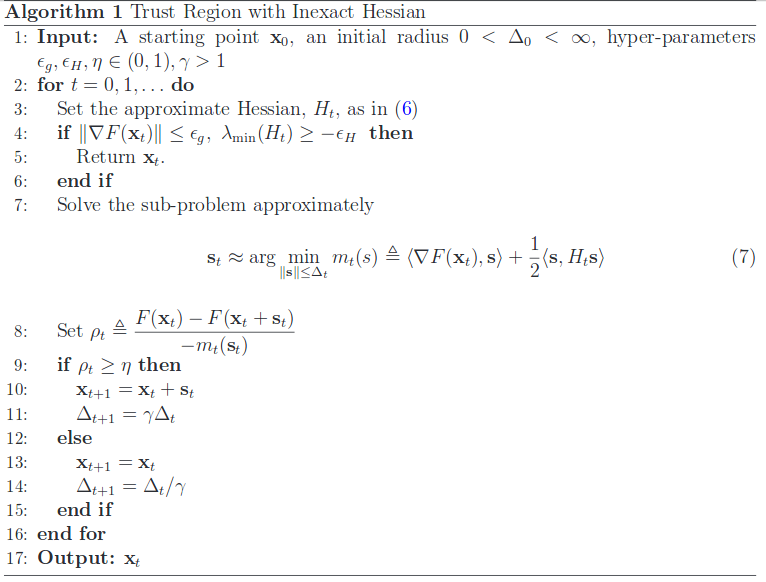
\includegraphics[width=0.9\textwidth]{./images/algo-1.png}
\column{0.55\textwidth}
\begin{theorem}
Consider any \(0 < \eg, \eh < 1\). Suppose
\begin{itemize}
\item<1->{\(H(\xbold)\) satisfies Inexact Hessian Regularity with \(\epsilon < (1 - \eta)\nu\eh\)}
\item<2->{\(\h F(\xbold)\) satisfies Hessian regularity}
\item<3->{if the approximate solution to \ref{TR} satisfies Sufficient Descent Condition-1}, 
\uncover<4->{then the algorithm terminates in at most \(T = O\left(\max\{\eh^{-1}\eg^{-2}, \eh^{-3}\}\right)\) iterations}
\end{itemize}
\end{theorem}
\end{columns}
\end{frame}

\begin{frame}{Conditions on the Inexact Hessian}
\begin{alertblock}{Sufficient Descent Condition-2}
Assume that we solve \ref{CR} approximately to find \(\sbold_{t}\) such that:
\begin{itemize}
\item \(-m_{t}(\sbold_{t}) \geq -m_{t}(\sbold_{t}^{C}) \geq \max\lbrace\Phi_{2}(\sigma_{t}, \sbold_{t}, B_{H}, \g F(\xbold_{t})), \Psi_{2}(\sigma_{t}, B_{H}, \g F(\xbold_{t}))\rbrace\)
\item \(-m_{t}(\sbold_{t}) \geq -m_{t}(\sbold_{t}^{C}) \geq \frac{\nu|\mineig(H_{t})|}{6} \max\lbrace ||\sbold_{t}^{E}||^{2}, \frac{\nu^{2}|\mineig(H_{t})|^{2}}{\sigma_{t}^{2}}\rbrace \text{ if } \mineig(H_{t}) < 0\)
\end{itemize}
\(\sbold_{t}^{C}\) is a Cauchy point, along the negative gradient direction and \(\sbold_{t}^{E}\) is along negative curvature direction such that \((\sbold_{t}^{E})^{T} H_{t} \sbold_{t}^{E} \leq \nu\mineig(H_{t})||\sbold_{t}^{E}||^{2} < 0\) for some \(\nu \in (0, 1]\).
\end{alertblock}
\pause
\begin{alertblock}{Sufficient Descent for Optimal Complexity}
Assume that we solve \ref{CR} approximately to find \(\sbold_{t}\) such that:
\[||\nabla m_{t}(\sbold_{t})|| \leq \theta_{t}||\g F(\xbold_{t})||, \hspace{4mm} \text{ where }\theta_{t} = \zeta\min\{1, ||\sbold_{t}||\} \text{ and } \zeta \in (0, 1) \]
\end{alertblock}
\end{frame}

\begin{frame}{Algorithm for Cubic Regularization method}
\begin{columns}
\column{0.45\textwidth}
\centering
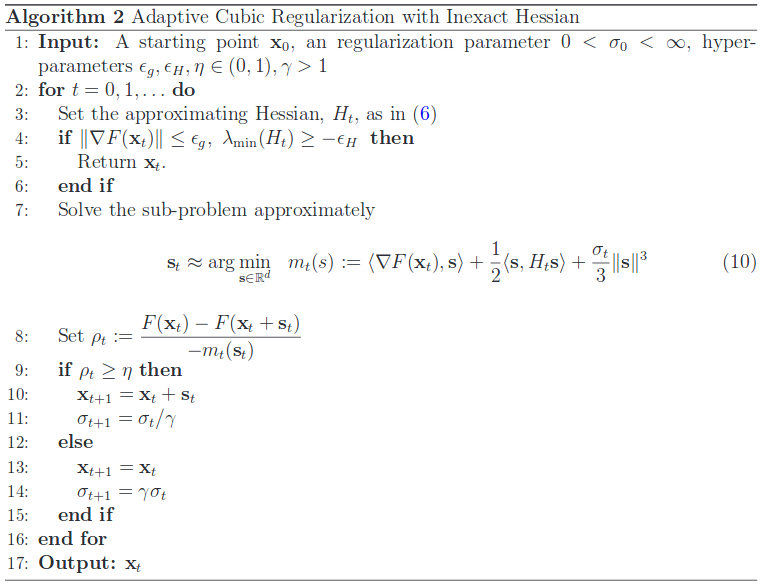
\includegraphics[width=0.9\textwidth]{./images/algo-2.png}
\column{0.55\textwidth}
\begin{theorem}
Consider any \(0 < \eg, \eh < 1\). Suppose
\begin{itemize}
\item<1->{\(H(\xbold)\) satisfies Inexact Hessian Regularity with \(\epsilon = \min\{\epsilon_{0}, \zeta \eg\}, \zeta \in (0, 0.5)\)}
\item<2->{\(\h F(\xbold)\) satisfies Hessian regularity}
\item<3->{if the approximate solution to \ref{CR} satisfies Sufficient Descent Condition-2 and Sufficient Descent for Optimal Complexity}, 
\uncover<4->{then the algorithm terminates in at most \(T = O\left(\max\{\eg^{-3/2}, \eh^{-3}\}\right)\) iterations}
\end{itemize}
\end{theorem}
\end{columns}
\end{frame}

\begin{frame}{Characteristics of Inexact Hessian in these methods}
\begin{itemize}
\item<1->{Same convergence rates with actual Hessians}
\item<2->{Both the methods - trust region and cubic regularization, at termination satisfy
  \begin{equation*}
  ||\g F(\xbold_{T})|| \leq \eg \hspace{4mm} \text{ and } \hspace{4mm} \mineig(\h F(\xbold_{T})) \geq -(\eh + \epsilon)
  \end{equation*}
  \uncover<3->{in terms of the optimal point definition, these are \((\eg, \eh + \epsilon)\)-optimal points}
} 
\end{itemize}
\end{frame}

\section{Finite-Sum Minimization}
\subsection{Random Sub-sampling}
\begin{frame}{General problem}
\begin{itemize}
\item<1->{Consider a modified unconstrained optimization problem
  \begin{equation}
    \min_{\xbold \in \mathbb{R}^{d}} F(\xbold) \triangleq \frac{1}{n}\displaystyle \sum_{i=1}^{n} f_{i}(\xbold)
  \end{equation}
where each \(f_{i}\) is smooth, but possibly non-convex.}
\item<2->{Seen in Machine Learning problems, where each \(f_{i}\) corresponds to the loss or mis-fit due to the \(i^{th}\) sample in the mini-batch/batch}
\item<3->{Large-scale problems have \(n, d >> 1\).}
\item<4->{Consider a probability distribution over \({1, 2, \ldots, n}\), denoted by \(\mathbf{p} = \{p_{i}\}_{i=1}^{n}\) and \(Pr(X = i) = p_{i} > 0, \hspace{2mm} \sum p_{i} = 1\). Based on \(\mathbf{p}\), we pick a sample \(\mathcal{S}\).}
\item<5->{Define the sub-sampled Hessian to be:
  \begin{equation}
    H(\xbold) \triangleq \frac{1}{n|\mathcal{S}|}\sum_{j \in \mathcal{S}} \frac{1}{p_{j}} \h f_{j}(\xbold)
  \end{equation}
}
\end{itemize}
\end{frame}

\begin{frame}{General problem - Uniform sampling of the Hessian}
\begin{theorem}
Consider \(\displaystyle \sup_{\xbold\in\mathbb{R}^{d}} ||\h f_{i}(\xbold)|| \leq K_{i}, \hspace{2mm} \forall i \in \{1, 2, \ldots, n\}\). Let \(\displaystyle K_{\max} = \max_{i=1,\ldots, n} K_{i}\). If \(p_{i} = \frac{1}{n} \hspace{1mm} \forall i \in \{1, 2, \ldots, n\}\), and \(|\mathcal{S}| \geq \frac{16K^{2}_{max}}{\epsilon^{2}}\log\frac{2d}{\delta} \), then with probability at least \(1 - \delta\), we have:
\begin{equation}
Pr\left(||H(\xbold) - \h F(\xbold)|| \leq \epsilon\right) \geq 1 - \delta
\end{equation}
\end{theorem}
\pause
\uncover<2->{Some major implications:}
\begin{itemize}
\item<3->{Higher the value of \(d\), more larger sample set is required. But this dependence is logarithmic.}
\item<4->{Higher the number of samples, lower the value of \(\epsilon\), in turn better ``inexact'' Hessian.}
\end{itemize}
\end{frame}

\begin{frame}{Special sub-problem}
\begin{itemize}
\item<1->{Applying a minor modification \(\xbold \rightarrow \mathbf{a}_{i}^{T}\xbold\), redefine the unconstrained optimization problem
  \begin{equation}
    \min_{\xbold \in \mathbb{R}^{d}} F(\xbold) \triangleq \frac{1}{n}\displaystyle \sum_{i=1}^{n} f_{i}(\mathbf{a}_{i}^{T}\xbold)
  \end{equation}
where each \(f_{i}\) is smooth, but possibly non-convex.}
\item<2->{Provides a more clear analogy to Machine Learning problems, where \(\mathbf{a}_{i}\) is a ``data-vector" e.g., Linear Kernel SVMs, Logistic Regression}
\item<3->{\(\h F(\xbold) = \frac{1}{n} \displaystyle \sum_{i=1}^{n} f_{i}''(\mathbf{a}_{i}^{T}\xbold) \mathbf{a}_{i}\mathbf{a}_{i}^{T}\)}
\end{itemize}
\end{frame}

\begin{frame}{Special sub-problem - Non-uniform sampling of the Hessian}
\begin{theorem}
Consider \(\displaystyle \sup_{\xbold\in\mathbb{R}^{d}} ||\h f_{i}(\xbold)|| \leq K_{i}, \hspace{2mm} \forall i \in \{1, 2, \ldots, n\}\). Let \(\hat{K} = \frac{1}{n}\sum_{i=1}^{n} K_{i}\). If \(p_{i} = \displaystyle \frac{|f_{i}''(\mathbf{a}_{i}^{T}\xbold)| ||\mathbf{a}_{i}||^{2}_{2}}{N}\), where \(N\) is a normalizing factor and \(|\mathcal{S}| \geq \frac{4\hat{K}^{2}}{\epsilon^{2}}\log\frac{2d}{\delta}\), then with probability at least \(1 - \delta\), we have:
\begin{equation}
Pr\left(||H(\xbold) - \h F(\xbold)|| \leq \epsilon\right) \geq 1 - \delta
\end{equation}
\end{theorem}
\pause
\uncover<2->{Some major implications:}
\begin{itemize}
\item<3->{Higher the value of \(d\), more larger sample set is required. But this dependence is logarithmic.}
\item<4->{Higher the number of samples, lower the value of \(\epsilon\), in turn better ``inexact'' Hessian.}
\item<5->{Probabilities are also determined by the ``length" of the data.}
\end{itemize}
\end{frame}

\begin{frame}{Usefulness and general ideas presented by these bounds}
\begin{itemize}
\item<1->{Both bounds depend on \(d\) in a logarithmic sense.}
\item<2->{Larger the size of \(\mathcal{S}\), better the ``inexact" Hessian.
  \begin{itemize}
    \item<3->{\(\hat{K} \leq K_{\max}\). So?}
    \item<4->{Smaller sample size \(|\mathcal{S}|\) required to achieve same level of accuracy in non-uniform sampling compared to uniform sampling}
    \item<5->{Proves helpful if distribution of \(K_{i}'s\) is skewed i.e., \(\hat{K} << K_{\max}\)}
  \end{itemize}
}
\item<3->{Choice of samples depend on the amount of curvature \(f_{i}''(\mathbf{a}_{i}^{T}\xbold)\), higher curvature \(\implies\) higher probability of being sampled.}
\end{itemize}
\end{frame}

\subsection{Convergence Analysis of Finite-Sum Minimization}
\begin{frame}{Probabilistic Convergence for Trust Region on Finite-Sum Minimization}
\begin{theorem}
Consider \(0 < \eg, \eh < 1\).
\begin{itemize}
\item<1->{\(H(\xbold)\) satisfies Inexact Hessian Regularity with \(\epsilon < (1- \eta)\nu\eh\)}
\item<2->{\(\h F(\xbold)\) satisfies Hessian regularity}
\item<3->{\(\delta_{0} = \delta\min\{\eg^{2}\eh, \eh^{3}\}\) for some \(\delta \in (0, 1)\)}
\item<4->{\(\mathcal{S}\) sampled with parameters \(\epsilon, \delta_{0}\) using either uniform or non-uniform sampling.}
\item<5->{if the approximate solution to \ref{TR} satisfies Sufficient Descent Condition-1, \uncover<6->{then the algorithm terminates in at most \(T = O\left(\max\{\eh^{-1}\eg^{-2}, \eh^{-3}\}\right)\) iterations, and with probability \(1 - \delta\), \(||\g F(\xbold_{T})|| \leq \eg \hspace{4mm} \text{ and } \hspace{4mm} \mineig(\h F(\xbold_{T})) \geq -(\epsilon + \eh)\).}}
\end{itemize}
\end{theorem}
\end{frame}

\begin{frame}{Probabilistic Convergence for Cubic Regularization on Finite-Sum Minimization}
\begin{theorem}
Consider \(0 < \eg, \eh < 1\).
\begin{itemize}
\item<1->{\(H(\xbold)\) satisfies Inexact Hessian Regularity with \(\epsilon = \min\{\epsilon_{0}, \zeta\eg\}, \zeta \in (0, 0.5)\)}
\item<2->{\(\h F(\xbold)\) satisfies Hessian regularity}
\item<3->{\(\delta_{0} = \delta\min\{\eg^{3/2}, \eh^{3}\}\) for some \(\delta \in (0, 1)\)}
\item<4->{\(\mathcal{S}\) sampled with parameters \(\epsilon, \delta_{0}\) using either uniform or non-uniform sampling.}
\item<5->{if the approximate solution to \ref{CR} satisfies Sufficient Descent Condition-2 and Sufficient Descent for Optimal Complexity, \uncover<6->{then the algorithm terminates in at most \(T = O\left(\max\{\eg^{-3/2}, \eh^{-3}\}\right)\) iterations, and with probability \(1 - \delta\), \(||\g F(\xbold_{T})|| \leq \eg \hspace{4mm} \text{ and } \hspace{4mm} \mineig(\h F(\xbold_{T})) \geq -(\epsilon + \eh)\).}}
\end{itemize}
\end{theorem}
\end{frame}

\section{Conclusion}
\begin{frame}{Summary}
\begin{itemize}
\item<1->{Approximation of curvature information}
\item<2->{Introduction to Trust Region and Cubic Regularization}
\item<3->{Achieving approximate optimality based on conditions or properties of the inexact Hessian}
\item<4->{Introduction to subsampling strategies}
\item<5->{Probabilistic convergence for Trust Region and Cubic Regularization on the finite-sum minimization problem}
\item<6->{Very theoretical - please view \href{arxiv.org/abs/1708.07827}{\beamergotobutton{Second-Order Optimization for Non-Convex Machine Learning: An Empirical Study}}}
\end{itemize}
\end{frame}

\begin{frame}{Questions??}
\end{frame}

\begin{frame}[t,allowframebreaks]
\frametitle{References}
\bibliographystyle{plain}
\bibliography{main.bib}
\end{frame}
\end{document}
